\documentclass[../main.tex]{subfiles}
\begin{document}

\problem{1}
Draw the state diagrams for the finite-state machine with these state tables
\begin{enumerate}[a)]
	\setcounter{enumi}{1}
	\item 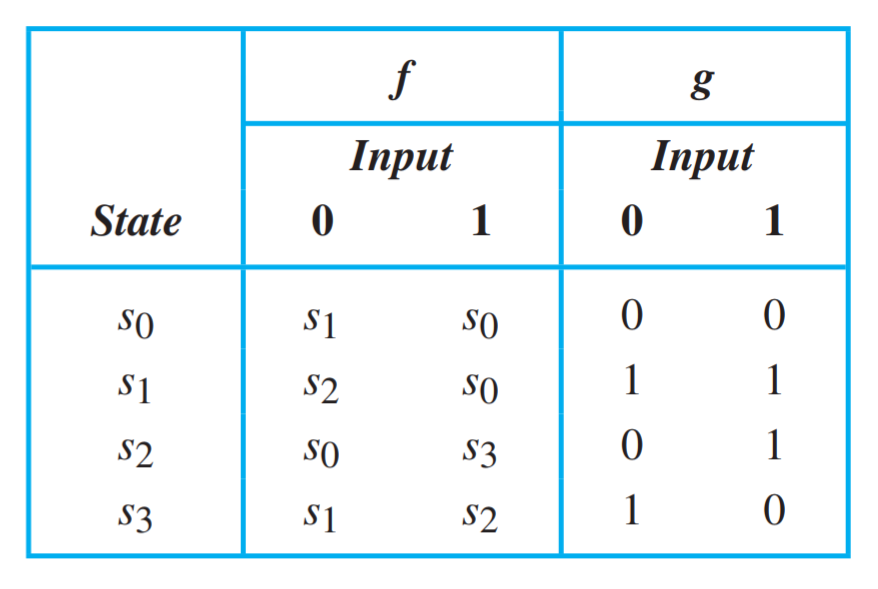
\includegraphics[width=\textwidth]{img/1bA.png}
\end{enumerate}

\solution
\begin{enumerate}[a)]
	\setcounter{enumi}{1}
	\item

\begin{center}
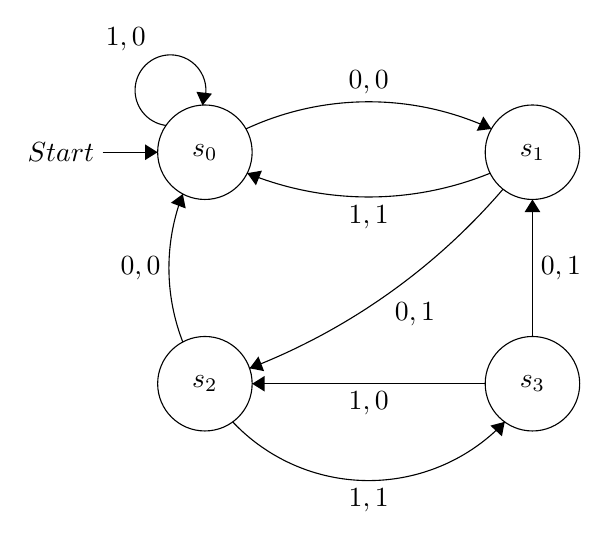
\begin{tikzpicture}[scale=0.2]
\tikzstyle{every node}+=[inner sep=0pt]
\draw [black] (22.1,-21.5) circle (3);
\draw (22.1,-21.5) node {$s_0$};
\draw [black] (42.9,-21.5) circle (3);
\draw (42.9,-21.5) node {$s_1$};
\draw [black] (22.1,-36.2) circle (3);
\draw (22.1,-36.2) node {$s_2$};
\draw [black] (42.9,-36.2) circle (3);
\draw (42.9,-36.2) node {$s_3$};
\draw [black] (15.6,-21.5) -- (19.1,-21.5);
\draw (15.1,-21.5) node [left] {$Start$};
\fill [black] (19.1,-21.5) -- (18.3,-21) -- (18.3,-22);
\draw [black] (24.706,-20.02) arc (114.94743:65.05257:18.479);
\fill [black] (40.29,-20.02) -- (39.78,-19.23) -- (39.36,-20.14);
\draw (32.5,-17.8) node [above] {$0,0$};
\draw [black] (40.214,-22.831) arc (-67.84225:-112.15775:20.454);
\fill [black] (24.79,-22.83) -- (25.34,-23.6) -- (25.72,-22.67);
\draw (32.5,-24.84) node [below] {$1,1$};
\draw [black] (19.643,-19.8) arc (263.0546:-24.9454:2.25);
\draw (17.08,-15.1) node [above] {$1,0$};
\fill [black] (21.95,-18.52) -- (22.55,-17.78) -- (21.56,-17.66);
\draw [black] (41.031,-23.846) arc (-40.66555:-68.8344:40.497);
\fill [black] (24.94,-35.22) -- (25.86,-35.4) -- (25.5,-34.47);
\draw (35.44,-31.03) node [below] {$0,1$};
\draw [black] (20.699,-33.555) arc (-158.72823:-201.27177:12.968);
\fill [black] (20.7,-24.15) -- (19.94,-24.71) -- (20.88,-25.07);
\draw (19.32,-28.85) node [left] {$0,0$};
\draw [black] (41.14,-38.619) arc (-43.27943:-136.72057:11.867);
\fill [black] (41.14,-38.62) -- (40.23,-38.86) -- (40.96,-39.54);
\draw (32.5,-42.85) node [below] {$1,1$};
\draw [black] (42.9,-33.2) -- (42.9,-24.5);
\fill [black] (42.9,-24.5) -- (42.4,-25.3) -- (43.4,-25.3);
\draw (43.4,-28.85) node [right] {$0,1$};
\draw [black] (39.9,-36.2) -- (25.1,-36.2);
\fill [black] (25.1,-36.2) -- (25.9,-36.7) -- (25.9,-35.7);
\draw (32.5,-36.7) node [below] {$1,0$};
\end{tikzpicture}
\end{center}
\end{enumerate}

\end{document}
